\renewcommand{\proofname}{Доведення}
\renewcommand{\chaptername}{РОЗДІЛ}


\chapter{Огляд теоретичної частини розробки з крос-платформеними фреймворками}
\label{ch1}


\section{Тренди серед мобільних фреймворків}
\label{sec:trends}

\subsection{Розробка крос-платформних мобільних додатків}
\label{subsec:cross_platform_dev}
Завдяки міжплатформенній розробці підприємства та організації змогли охопити ширшу аудиторію, ефективніше та з меншими витратами.
React Native був представлений Facebook у 2015 році.
React Native - це фреймворк для мобільних додатків з відкритим кодом, який використовує React із власними можливостями платформи для розробки додатків для Android, iOS, Web та UWP.

Список компаній, що використовують React Native в своїх мобільних додатках: Facebook, Instagram, Tesla, Uber Eats, Discord, Wix, Walmart.

Компетентний розробник React Native повинен знати JavaScript + React Native SDK, Kotlin + Android SDK, Swift + iOS SDK, що в 3 рази більше знань у порівнянні зі звичайними розробниками мобільних пристроїв.
Звідси відсутність хороших розробників та підвищеня ціни розробки майже у 3 рази.
Якщо ви вирішите використовувати React Native треба розважити це рішення, оскільки для переходу на інші кроссплатформенні
фреймворки потребує повну переробку коду додатку.

Flutter був представлений Google у травні 2017 року. Але випуск стабільної версії відбувся у грудні 2018 року.
Flutter також має відкритий вихідний код і використовується для розробки програм для Android, iOS, Linux, Mac, Windows, Google Fuchsia та веб.

Деякі програми, створені за допомогою Flutter, це: Google Ads, Alibaba.com, Realtor.com.

Оскільки Flutter та React-Native стали найгарячішою темою останніх днів
та конкурентними дебатами серед спільноти розробників, багато розробників залижаються у невизначеності, визначаючи, яку платформу вибрати.

Flutter eкосистема ще не настільки зріла, як в випадку React Native, але швидко розвивається.
Власні бібліотеки та код можна інтегрувати з програмами Flutter, тому, так само як і в React Native,
тут потрібні знання SDK нативних платформ iOS та Android.
Знову та сама проблема з 3 мовами, що вимагає від розробників одночасного володіння Flutter SDK, iOS SDK та Android SDK.
Оскільки Flutter використовує Dart, а фреймворк написаний майже з нуля,
розробникам буде важко перенести проекти Flutter на інші крос-платформні фреймворки або власні програми.
Як і в випадку React Native потрібно буде переписати все з нуля.

Цільова аудиторія Kotlin Multiplatform - це нативні розробники мобільних платформ, які вже використовують Kotlin на Android та Swift на iOS.
Іншими словами, це розробники, які глибоко розуміють рідні мобільні SDK, яким потрібно вивчити лише одну нову мову (Swift або Kotlin).
Таким чином, Kotlin Mutlitplatform потребує меньших інвестицій оскільки вони залишаються в той самій ніщі.
Головний недолік Kotlin Mutlitplatform - це те, що фреймфорк досі в Alpha версії. На період 5 травня 2021 це версія 0.2.4 (див. \cite{kmm_plugin_releases}).

\begin{center}
    \begin{longtable}{|p{0.23\textwidth}|p{0.22\textwidth}|p{0.22\textwidth}|p{0.23\textwidth}|}
        \caption{Порівняння Фреймворків}
        \label{tab:framwework_comparison}
        \\ \hline
        & React Native                               & Flutter                               & Kotlin Multiplatform                              \\
        \hline \endfirsthead
        \subcaption{Продовження таблиці~\ref{tab:framwework_comparison}}
        \\ \hline \endhead
        \hline \subcaption{Продовження на слід. стор.}
        \endfoot
        \hline \endlastfoot
        Вперше з’явився       & 2015                                & 2017                                & 2018                               \\
        \hline
        Розроблено                   & Facebook                         & Google                               & JetBrains                            \\
        \hline
        Відкрите джерело         & Так                                & Так                                & Так                               \\
        \hline
        Мова             & Javascript                           & Dart                           & Kotlin                               \\
        \hline
        Нативні Модулі & Так                      & Так                      & Так                             \\
        \hline
        Сумісність   & Обмежена & Обмежена & Так \\
        \hline
        Інші мови для вивчення                    & Kotlin, Swift                & Kotlin, Swift                     & Swift             \\
        \hline
        Клікість Розробників      & 42\%\cite{worldwide_sf_work_hours}                     & 39\%\cite{worldwide_sf_work_hours}                & 2\%\cite{worldwide_sf_work_hours}  \\
        \hline
        IDE      & Немає офіційної IDE                     & Android Studio                & Android Studio, XCode  \\
        \hline
        Цільова аудиторія      & Веб-розробники                     & Розробники флаттера                & Розробники під мобільні пристрої  \\
    \end{longtable}
\end{center}

\subsection{Тренди}
\label{subsec:mobile_trends}

\begin{figure}
    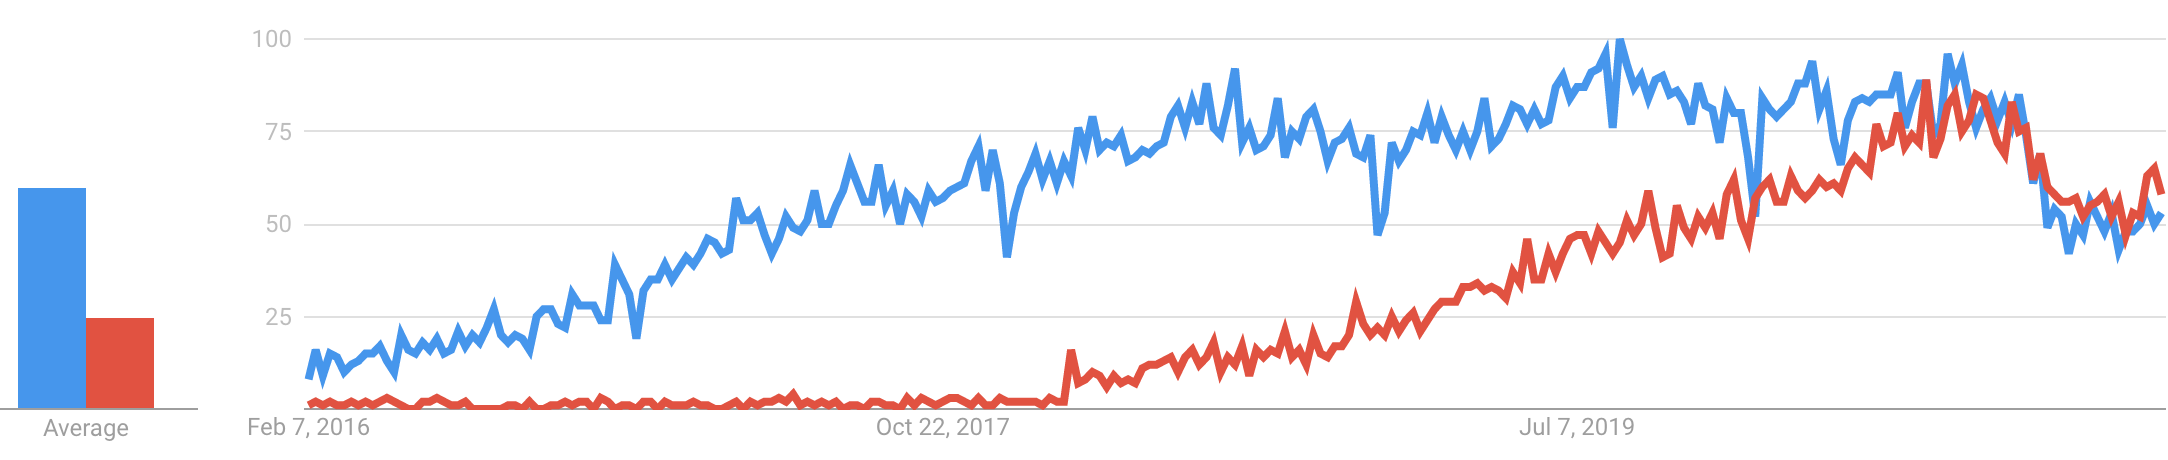
\includegraphics[width=\textwidth]{flutter_react_trend_5_years.png}
    \caption{Відповідно до Google Trends за 5 років}
    \label{fig:flutter_react_trend_5_years}
\end{figure}

На Google Trends за останні п’ять років Flutter випередив React Native (див. рис.~\ref{fig:flutter_react_trend_5_years}).
Але це не визначає, що Flutter - кращим варіантом в порівняні з React Native.

Порівнюючи тренди між Kotlin, Flutter та Reactive Native за 12 місяців також спостерігається більша зацікавленість Flutter.
Де Kotlin (див. рис.~\ref{fig:flutter_react_trend_12_months_1}) демонструє меньшу зацікавленість серед пошуків.
\begin{figure}
    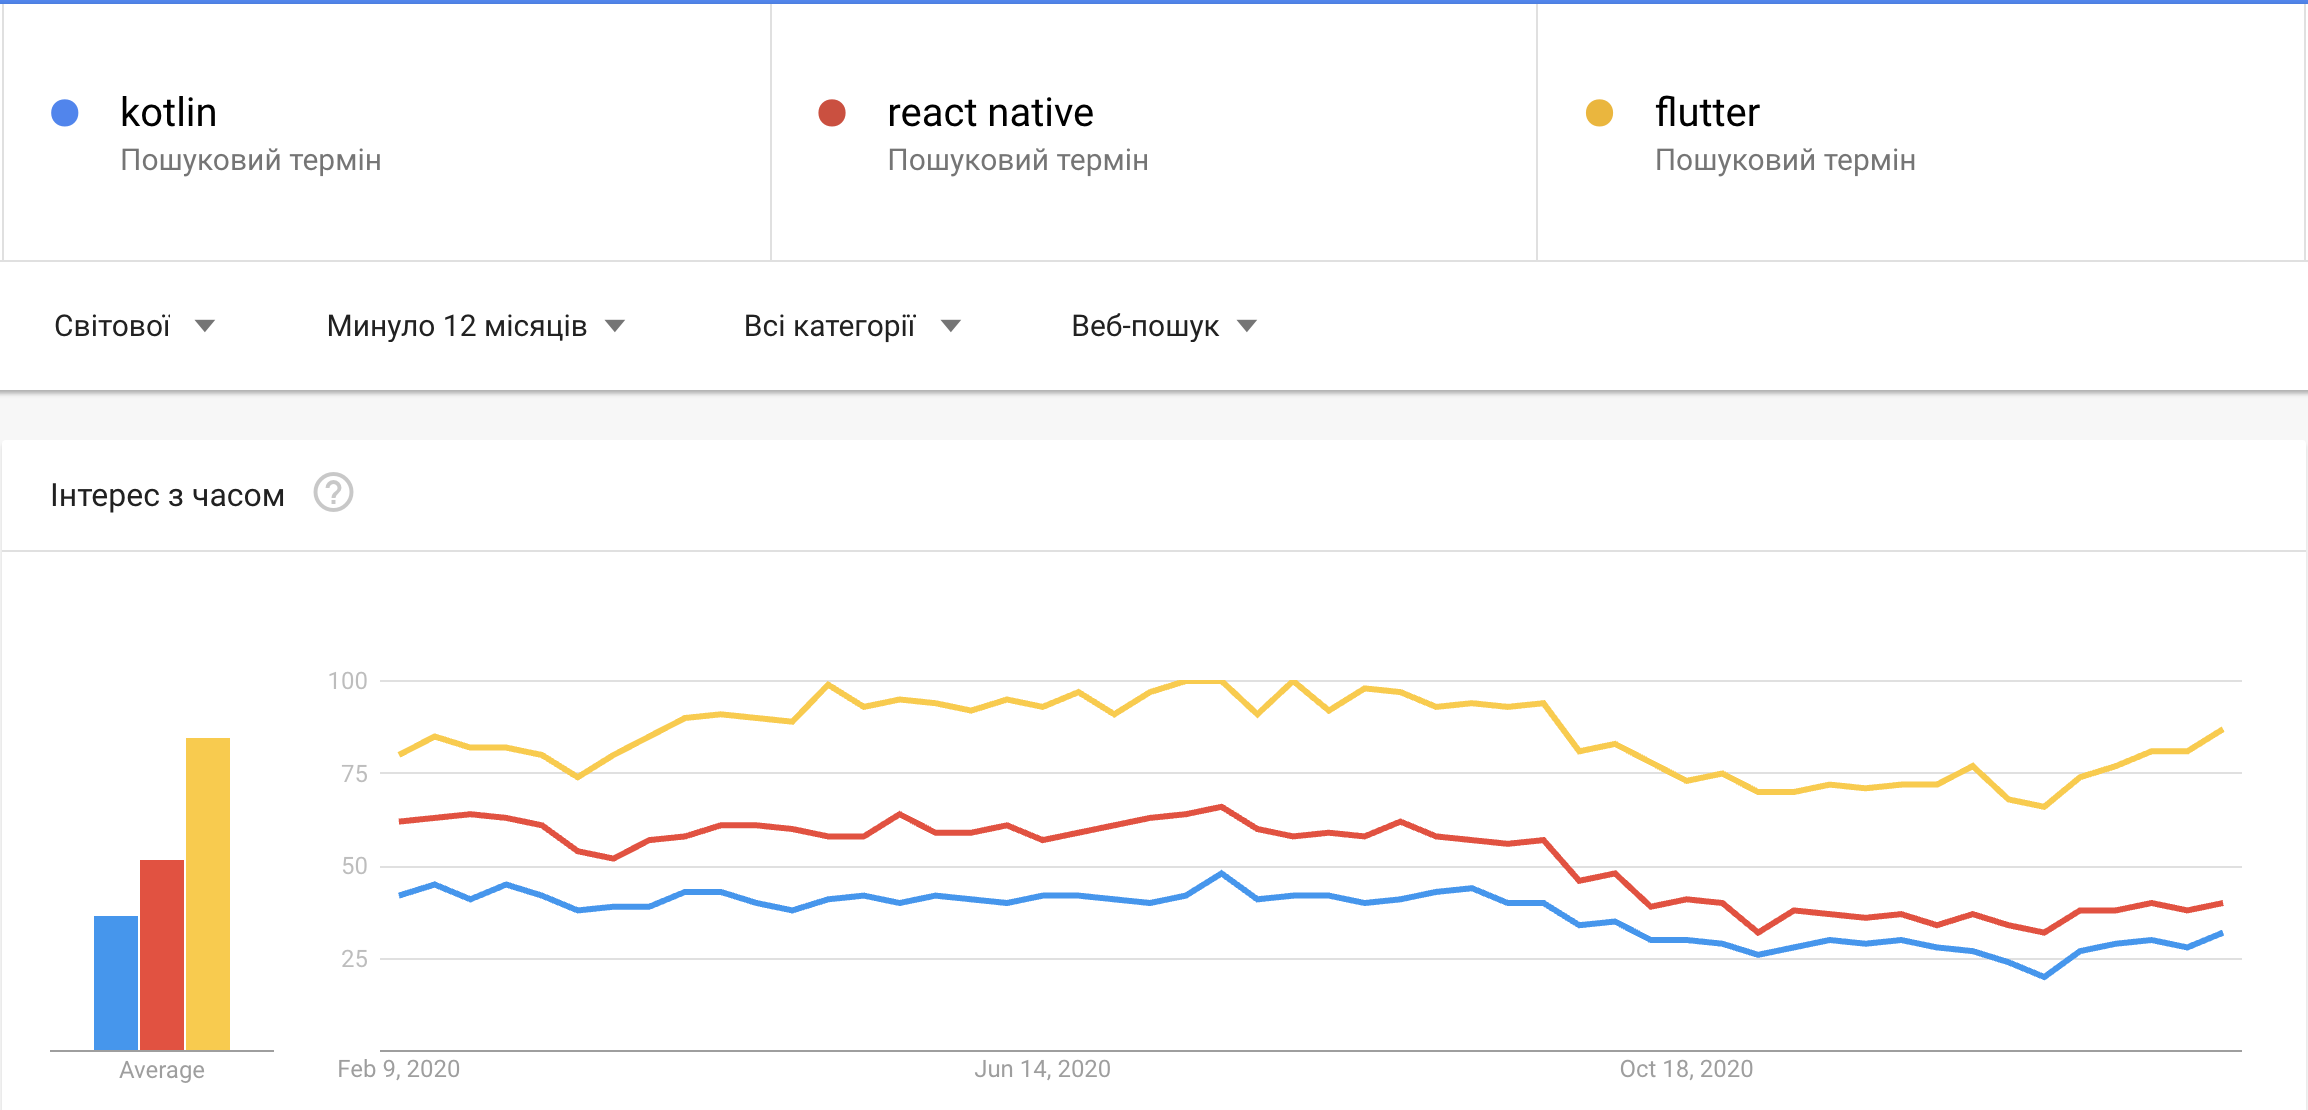
\includegraphics[width=\textwidth]{flutter_react_trend_12_months_1.png}
    \caption{Інтерес за часом Google Trends за 12 місяців \cite{google_trends}}
    \label{fig:flutter_react_trend_12_months_1}
\end{figure}

Оцінюючи мапу світу (див. рис.~\ref{fig:flutter_react_trend_12_months_2}) ми бачимо, що Flutter є лідером по зацікавленості сереж регіонів, коли React Native уступає всім трьом.
\begin{figure}
    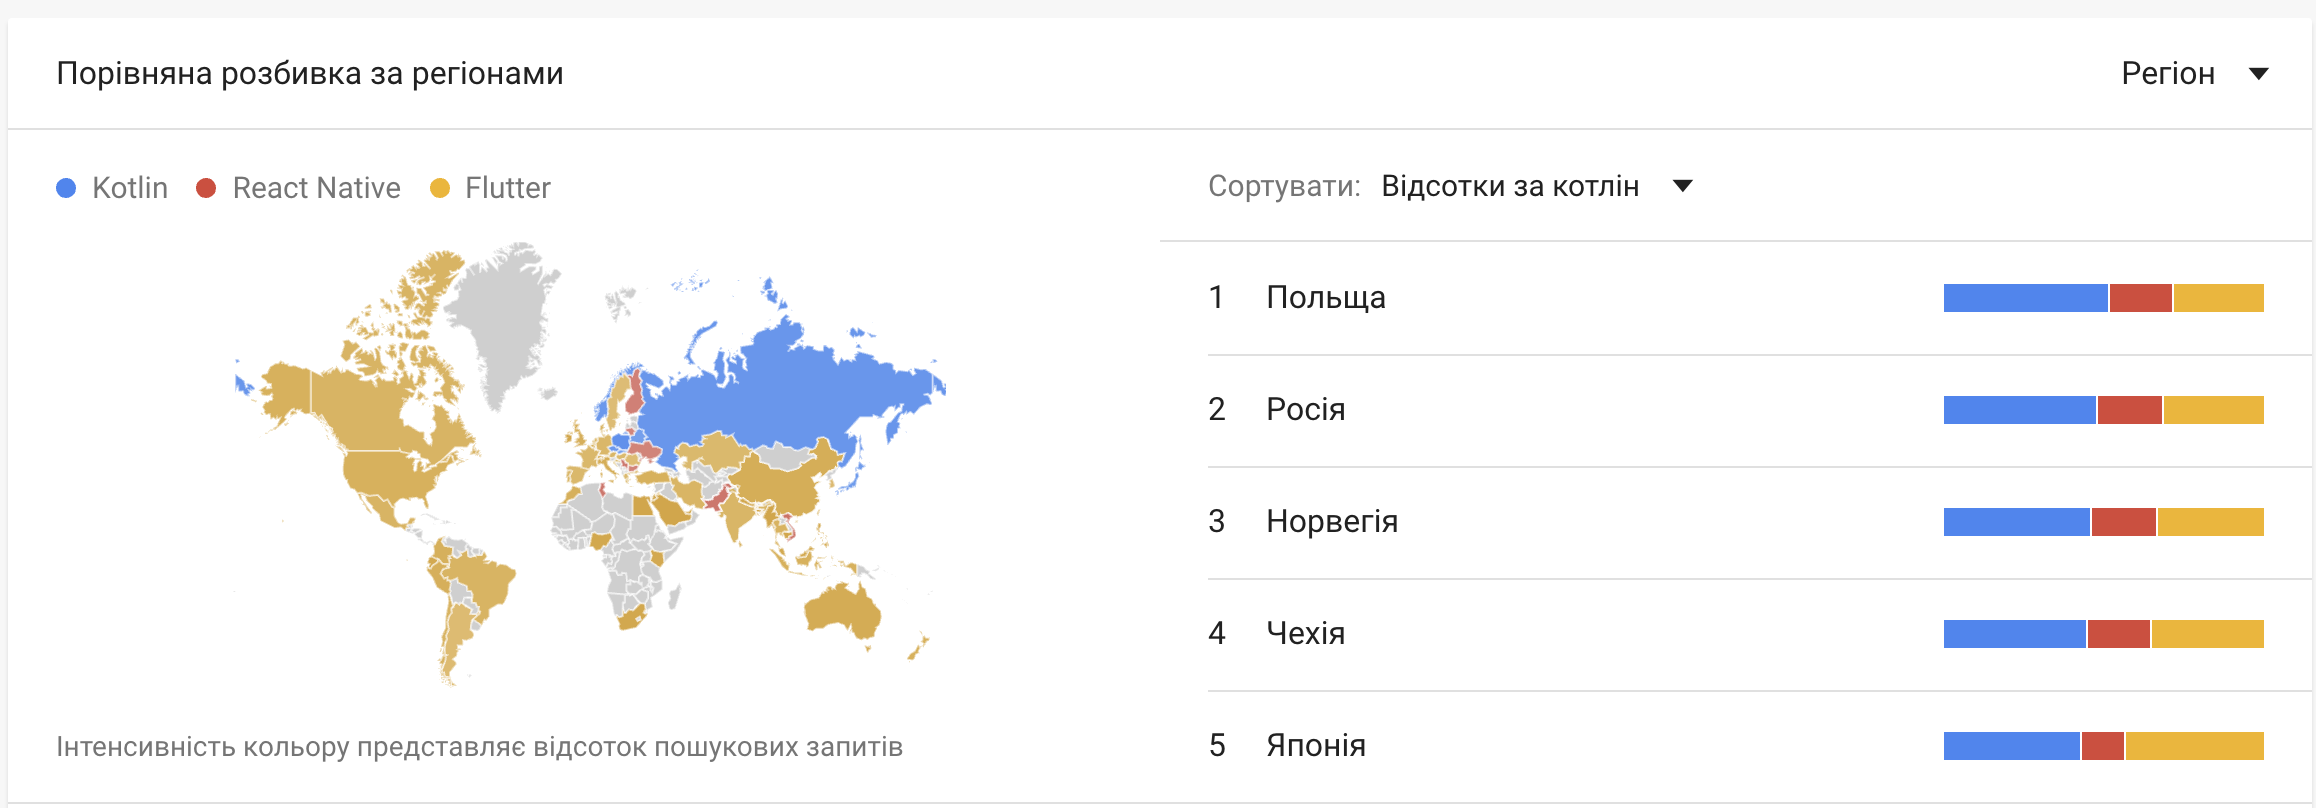
\includegraphics[width=\textwidth]{flutter_react_trend_12_months_2.png}
    \caption{Розподілення по регіонам \cite{google_trends}}
    \label{fig:flutter_react_trend_12_months_2}
\end{figure}

Якщо враховувати, тенденцій розвитку міжплатформенних технологій мобільних додатків, то і React Native, і Flutter досить схожі за популярністю.
Обидві технології посідають дуже високе місце на GitHub.
В лютому 2021 Flutter має 112 тис. зірок \cite{flutter_gihtub} та React Native 93.2 тис. \cite{rn_gihtub}.

Ми бачимо, що інтерес до Flutter значно зріс у 2021 році і швидко зростає.

\begin{figure}
    \begin{center}
        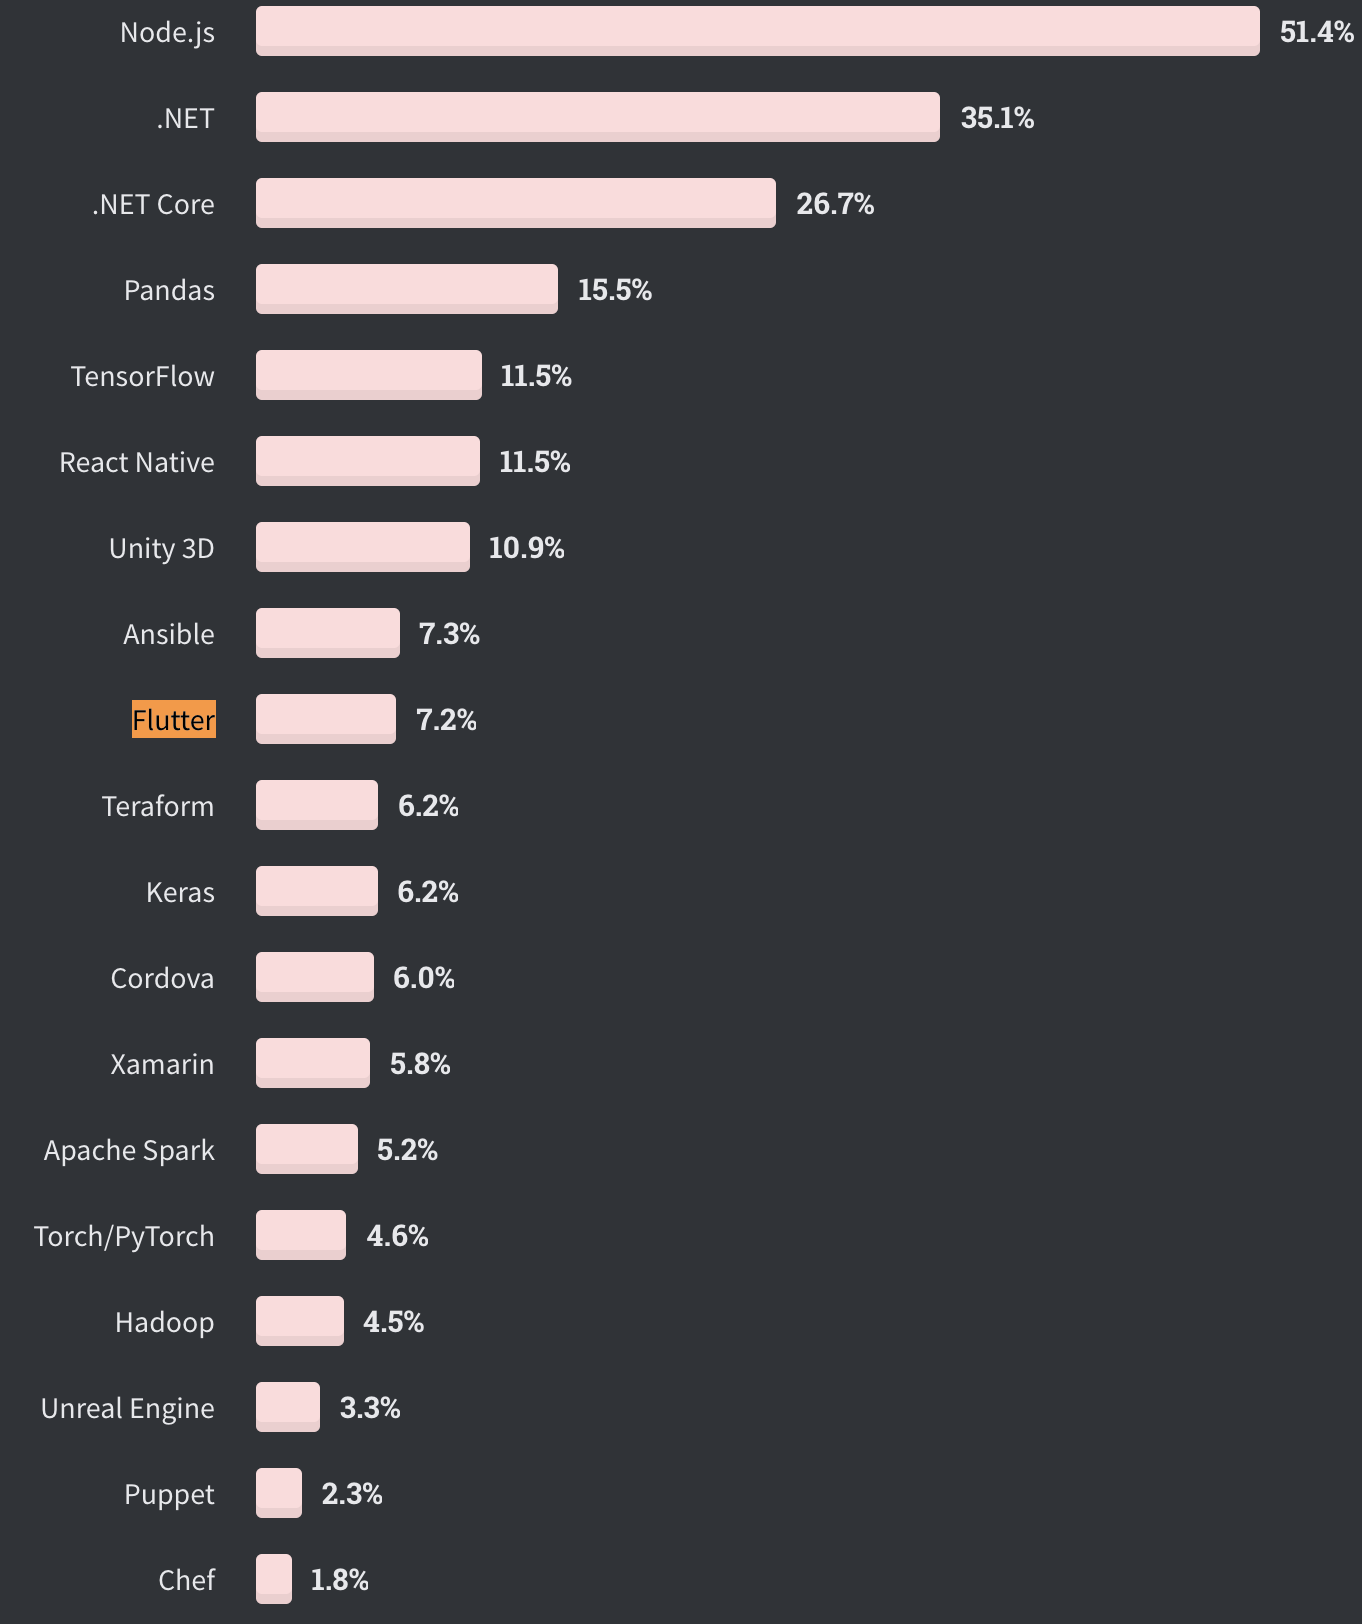
\includegraphics[scale=0.65]{stackoverflow_survey_2020.png}
    \end{center}
    \caption{Основна популярність за результатами опитування, яке охопило 40 000 відповідей. \cite{stackoverflow_survey_2020}}
    \label{fig:stackoverflow_survey_2020}
\end{figure}

\subsection{Переваги та недоліки Flutter}
\label{sec:flutter_pros_cons}

До переваг користування платформою Flutter можна віднести:
спільну кодову базу, потужна система віджетів, pixel perfect та hot reload можливості.

Flutter підтримує як мобільні платформи Android, так і iOS, і,
оскільки він відображає все самостійно, він дозволяє запускати все з однієї кодової бази.

У Flutter користувальницький інтерфейс побудований за допомогою віджетів,
невеликих будівельних блоків інтерфейсу, зібраних за допомогою техніки, що називається композиція.
Весь процес схожий на використання компонентів React.
Існує два набори віджетів, що доступні: Material Design, який сумісний з дизайнерськими вказівками Google,
та Cupertino, сумісний з Apple's вказівками для iOS.

Flutter управляє кожним пікселем екрану, тому ми можемо бути впевнені, що наші віджети будуть виглядати
однаково на всіх мобільних пристроях. Це, в свою чергу, дозволяє нам створювати дивовижні на вигляд
користувальницькі інтерфейси, які виглядають абсолютно однаково як на Android, так і на iOS.

Функція hot reload (гарячого перезавантаження) забезпечує можливість внесення змін на "льоту", дозволяючи бачити їх відразу під час розробки.
Ця функція мінімізує час очікування на результат змін під час розробки.

До недоліків користування платформою Flutter можна віднести:
відсутність підтримки смарт годиників та ТВ платформ,
затримки в підтримуванні найновших можливостей рідних платформ.

Flutter SDK не підтримує компоненти сумісні зі специфікаціями Apple TV та Android TV.

Функції, що нещодавно додані до систем iOS та Android, будуть адаптовані у Flutter пізніше, ніж у їхніх рідних версіях.

\begin{longtable}[c]{|l|l|}
    \caption{Переваги та недоліки Flutter.}
    \label{tab:rn_db_comparison}\\
    \hline
    Переваги &
    Недоліки \\ \hline
    \endhead
%
    Спільна кодова база. &
    \begin{tabular}[c]{@{}l@{}}Відсутність підтримки смарт\\ годиників та ТВ платформ.\end{tabular} \\ \hline
    \begin{tabular}[c]{@{}l@{}}Красиві інтерфейси\\ в найкоротші терміни.\end{tabular} &
    \begin{tabular}[c]{@{}l@{}}Затримки в підтримуванні \\ найновших можливостей \\ рідних платформ\end{tabular} \\ \hline
    Pixel perfect. &
    \begin{tabular}[c]{@{}l@{}}Більше використання\\ RAM та CPU.\end{tabular} \\ \hline
    \begin{tabular}[c]{@{}l@{}}Hot reload\\ (гаряче перезавантаження).\end{tabular} &
    Більший розмір додатку. \\ \hline
    Відкритий сирцевий код &
    \\ \hline
\end{longtable}

\subsection{Переваги React Native}
\label{subsec:rn_pros}
\begin{enumerate}
    \begin{item}
        Це зрілий фреймворк зі стабільним API, який підтримується Facebook.
    \end{item}
    \begin{item}
        Розробники додатків на React для веб можуть перевикористати набутий досвід, а тому легше буде перейти на нову платформу.
    \end{item}
    \begin{item}
        Так само, як Flutter, він дозволяє швидко розроблювати додатки iOS, Android та Web зі спільною кодовою базою.
    \end{item}
    \begin{item}
        React Native допомогає з управлінням стану при зміні конфігурацій часу виконання.
    \end{item}
\end{enumerate}

\subsection{Недоліки React Native}
\label{subsec:rn_cons}
\begin{enumerate}
    \begin{item}
        У ньому все ще бракує певних спеціальних модулів, специфічних для платформи, і для їх створення вам може знадобитися досвід native розробника.
    \end{item}
    \begin{item}
        Навігація не є плавною.
    \end{item}
    \begin{item}
        Міжплатформна розробка може спричинити проблеми з продуктивністю оскільки використовується додатковий рівень інтерпретації коду в runtime середовищі.
    \end{item}
    \begin{item}
        Це не найкращий вибір для програм, які потребують складну анімацію (на приклад ігри).
    \end{item}
\end{enumerate}

\subsection{Мови програмування}
\label{subsec:languages}

Flutter використовує мову, що називається Dart.
Це мова, яка має синтаксис, подібний до Java та Javascript.

Простим прикладом коду в Dart буде:
\begin{lstlisting}[style=light, language=Python,label={lst:vectorimg},caption=Dart Hello World]
void main () { 
  print ("Hello World!"); 
}
\end{lstlisting}

React Native використовує Javascript.
React Native побудований поверх React, який побудований на Javascript.
Тому, якщо вам доведеться вивчити React Native, вам знадобляться попередні знання Javascript.

Javascript існує довкола спільноти розробників програмного забезпечення дуже давно, і існує безліч ресурсів, на яких можна навчитися javascript.
Простим прикладом коду в javascript буде:

\begin{lstlisting}[style=light, language=Python,label={lst:vectorimg},caption=Dart Hello World]
  alert("Hello World!");
\end{lstlisting}

\subsection{Спільнота}
\label{subsec:communities}

Flutter і Dart були представлені спільноті розробників нещодавно, і порівняно, у неї менша спільнота розробників.
Google витратив багато на розробку Dart, і спільнота продовжує зростати.
Flutter має спільноти на StackOverflow, Slack та багатьох інших платформах.

React Native має більшу спільноту розробників, ніж Flutter, сприяючи його розвитку.
Спільнота Javascript є навіть більшою, ніж спільнота React Native, оскільки вона існує вже дуже давно, і допомогу можна знайти майже скрізь в Інтернеті.
Це, безумовно, пояснює, чому React Native має вищий рівень прийняття в порівнянні з Flutter.
Крім того, підтримка React, React Native та Javascript в Інтернеті є більш доступною.
Є мільйони рядків коду, які є у вільному доступі в Інтернеті, і їх можна просто «зняти» та використовувати у своїх проектах.
На сторінці спільноти React Native на їх офіційному веб-сайті вказані інші платформи, що вміщують їхні спільноти, такі як StackOverflow та Medium.

Найкраще у Dart - це те, що він постачається з повним набором віджетів інтерфейсу, які можна підняти прямо з коробки та використовувати.
В React Native, набір віджетів інтерфейсу мінімальний, і тому розробникам програмного забезпечення та програмістам доводиться звертатися до сторонніх бібліотек для віджетів інтерфейсу, і іноді їм доведеться створювати власні віджети інтерфейсу.

\subsection{Порівняння доступних вакансій на ринку Британії}
\label{subsec:market_comparisson}
Розглянемо статистичні дані, щодо популярності платформ на ринку праці.
В якості ринку праці був вибран останій на території Великої Британії, оскільки остання має досить розвиненний ринок IT.
За додаткову метрику розглянемо кількість вакансій доступних за остатні 6 місяців.

Отже вакансій доступних для React Native розробників 877, де 908 було за той самий період в 2020 і 750 за 2019 \cite{react_native_jobs}.
Вакансій на Flutter меньше всього 113 за 2021, 49 за 2020 та 12 за 2019 \cite{flutter_jobs}.
Враховуючи ці дані можна зробити висновок, що React Native показує більшу зацікавленість ринку праці.
Однак, в захист Flutter можна додати, що за остатній рік в рейтингу вакансій Flutter піднявся на 309 пунктів \cite{flutter_jobs}, коли React Native на 165 \cite{react_native_jobs}.

Нажаль схожої статистики по Kotlin Mutliplatform не вдалося точно виявити.
Загальна тенденція вакансій по Kotlin, як мові програмування показує нам 917 за 2021, 1 196 за 2020 та 644 за 2019 роки \cite{kotlin_jobs}.

Цікавим спостереженєм є медіана зарплат де Kotlin розробника пропонують £70,000\cite{kotlin_jobs}, React Native £60,000\cite{react_native_jobs} та Flutter £52,500\cite{flutter_jobs}.
Таку тенденцію можно пояснити широкопрофільним застосуванням Kotlin, як в розробці Backend так і Frontend клієнтів.


\section{Фреймворк React Native}
\label{sec:rn}

\subsection{Декларативність та React Native}
\label{subsec:rn_declarative}

React \textbf{декларативний} та спрощує створення інтерактивних інтерфейсів.
Вам потрібно лише описати, як різні частини інтерфейсу виглядають у кожному стані вашого додатку і React ефективно оновить та відрендерить лише потрібні компоненти.
Декларативні інтерфейси роблять наш код більш передбачуваним і його набагато легше налагоджувати.

React Native \textbf{заснований на інкапсульованих компонентах}, які керують власним станом, і з них будують складні інтерфейси.
Оскільки логіка компонентів написана на JavaScript, замість шаблонів, ми з легкістю можемo передавати складні дані у додатку і зберігати стан окремо від DOM.

Розглянемо оголошення змінної:
\begin{lstlisting}[style=light, language=Python,label={lst:jsx_hello},caption=JSX Hello World]
const element = <h1>Hello, world!</h1>;
\end{lstlisting}

Цей дивний синтаксис тегів не є ні рядком, ні HTML.

Він має назву \textbf{JSX}, і це розширення синтаксису для JavaScript.
Його використовує React, щоб описати інтерфейс користувача.
JSX може нагадувати мову шаблонів, але з усіма перевагами JavaScript.

React використовує той факт, що логіка виводу пов’язана з іншою логікою інтерфейсу користувача: як обробляються події, як змінюється стан з часом і як дані готуються для рендерингу.

Замість того, щоб штучно відокремити технології, розмістивши розмітку і логіку в окремих файлах, React розділяє відповідальність між вільно зв’язаними одиницями, що містять обидві технології і називаються "компонентами".
React не вимагає використання JSX, але більшість людей цінують його за візуальну допомогу при роботі з інтерфейсом користувача в коді JavaScript.
Він також дозволяє React показати зрозуміліші повідомлення про помилки та попередження.

\subsection{React та система побудування Expo}
\label{subsec:rn_expo}
React Native пропонує два різних способи побудування проекту \textbf{«керований»} та \textbf{«простий»} робочими процесами.
\begin{itemize}
    \begin{item}
        За допомогою \textbf{керованого} робочого процесу ви пишете лише інструменти та служби JavaScript / TypeScript та Expo, які піклуються про все інше.
    \end{item}
    \begin{item}
        У \textbf{простому} робочому процесі ви маєте повний контроль над кожним аспектом власного проекту, а інструменти та послуги Expo трохи більш обмежені.
    \end{item}
\end{itemize}

В обох випадках використовується екосистема інструментів, що спрощують процес пободування проекту, ховаючи деталі та називається Expo.
Expo - платформа для універсальних додатків React, набір інструментів та служб, побудованих навколо React Native та власних платформ, які допомагають вам розробляти, будувати, розгортати та швидко переглядати iOS, Android та веб-додатки з тієї самої кодової бази JavaScript / TypeScript.\cite{expo_doc}

\subsection{React та запити до мережі з Fetch API}
\label{subsec:rn_fetch_api}
React Native надає API Fetch для ваших мережевих потреб.
API Fetch забезпечує інтерфейс для отримання ресурсів (у тому числі по всій мережі).
Буде здаватися звичним кожному, хто використовував XMLHttpRequest, але новий API забезпечує більш потужний та гнучкий набір функцій.
Fetch забезпечує загальне визначення Requestі Responseоб'єктів (та інших речей, пов'язаних із мережевими запитами).
Це дозволить їх використовувати там, де вони потрібні в майбутньому.

Fetch API залежить від Promise.
Promise або "обіцянка" - це проксі для значення, яке не обов'язково відомо при створенні об'єкту.\cite{promise_doc}
Інакше кажучи, це API обгортка, яка задає контракт згідно которого promise(обіцянка) може знаходитись в одному зі станів:
A Promise знаходиться в одному з таких станів:
\begin{itemize}
    \begin{item}
        \textbf{в очікуванні(peding)}: початковий стан, ні виконаний, ні відхилений.
    \end{item}
    \begin{item}
        \textbf{виконано(fulfilled)} : це означає, що операція була успішно завершена.
    \end{item}
    \begin{item}
        \textbf{відхилено(rejected)} : означає, що операція не вдалася.
    \end{item}
\end{itemize}

Прикладом коду, котрий виконує запит та отримує відповідь в форматі JSON можна знайти в додатку \ref{lst:rn_network}.

\subsection{Realm React Native}
\label{subsec:rn_realm}
В випадку вибору бази даних треба розглянути наступні фактори:
\begin{itemize}
    \begin{item}
        \textbf{Технологія:} з відкритим кодом чи власністю?
    \end{item}
    \begin{item}
        \textbf{Архітектура:} SQL або NoSQL?s
    \end{item}
    \begin{item}
        \textbf{Масштабованість:} чи ви будете самостійно розміщувати або скористаєтесь масштабованою послугою?
    \end{item}
\end{itemize}

Ринок надає можливість використання таких рішень як:

\begin{longtable}[c]{|l|l|l|}
    \caption{Порівняння Баз Даниx React Native}
    \label{tab:rn_db_comparison} \\
    \hline
    & Сирцевий код  & Тип реаліаційної БД \\ \hline
    \endhead
%
    Back4app        & Відкритий     & SQL, NoSQL          \\ \hline
    Cloud Firestore & Пропрієтарний & NoSQL               \\ \hline
    DigitalOcean    & Відкритий     & SQL                 \\ \hline
    AWS RDS         & Відкритий     & SQL                 \\ \hline
    Realm           & Відкритий     & NoSQL               \\ \hline
\end{longtable}

Під час роботи над тестовим продуктом було зроблене рішення використати Realm.
Рішення базувалося скоріше на потребах швидкого та простого в інтеграції рішення.
Як наведено в додатку \ref{lst:rn_realm}  конфігурація в цілому є дуже проста (також див. \ref{fig:rn_realm}).

Спочатку ми описуємо схему бази даних. В даному випадку одна таблиця.
Створюємо об'єкт конфігурації, котрий буде використаний, щоби відкрити підключення до бази даних.
Передавши конфігурацію ми отримаємо відкрите підключення до бази даних та робимо запит до таблиці.
Запит повертає нам результат зі збереженими даним з котрих ми робимо копію кожного об\'єкту.
Особливість Realm об\'єктів полягає в тому, що вони є вікном до курсору в таблиці.
Щоби уникнути випадкових змін в таблиці ми спеціально робимо копію, яка є "чистим" об\'єктом від\'єднаним від БД.

\begin{figure}
    \begin{center}
        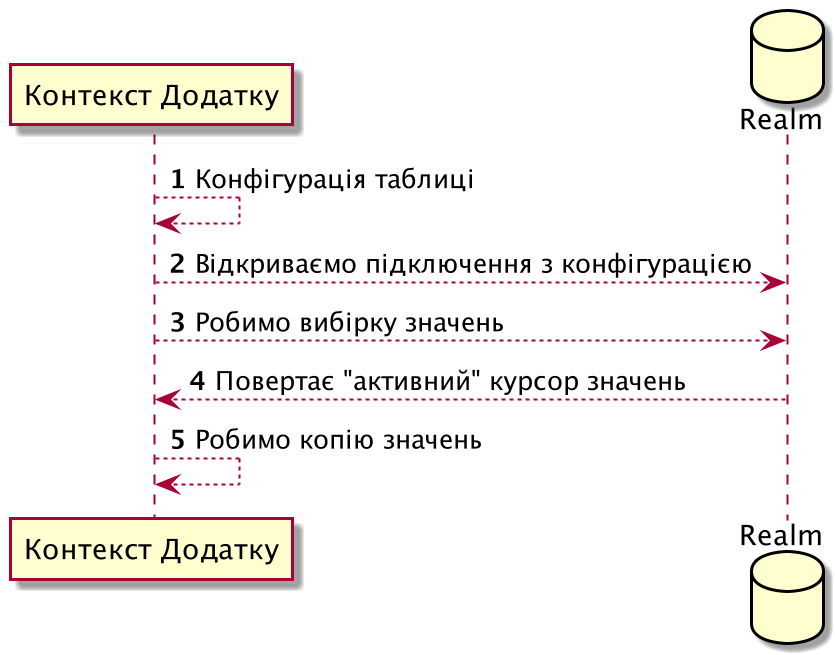
\includegraphics[scale=0.4]{rn_realm.png}
    \end{center}
    \caption{Взаємодія React Native додатку з БД}
    \label{fig:rn_realm}
\end{figure}

\subsection{React Native та управління станом}
\label{subsec:rn_state_management}

Даний підхід дозволяє швидко і в простий спосіб сконфігурувати стан нашого компоненту.
Хоч це і звучить просто нажаль, в більш складних компонентах з великою кількістю взаємодій з користувачем такий підхід призведе до високої зв'язаності коду.
В свою чергу ми отримаємо складний до зрозуміння сирцевий код і нестабільне рішення з великою кількістю помилок.
Для рішення цієї проблеми можна застосувати архітектуру Redux.

Redux - передбачуваний контейнер стану для Javscript додатків Apps (див. на \ref{fig:rn_realm}))..
Redux допомагає писати програми, які поводяться послідовно , працюють у різних середовищах (клієнтських, серверних та власних) і легкі для перевірки. \cite{redux_home_page}
Централізація стану та логіки вашого додатка забезпечує потужні можливості, такі як скасування / повтор , стійкість стану та багато іншого. \cite{redux_home_page}

\begin{center}
    \begin{figure}
        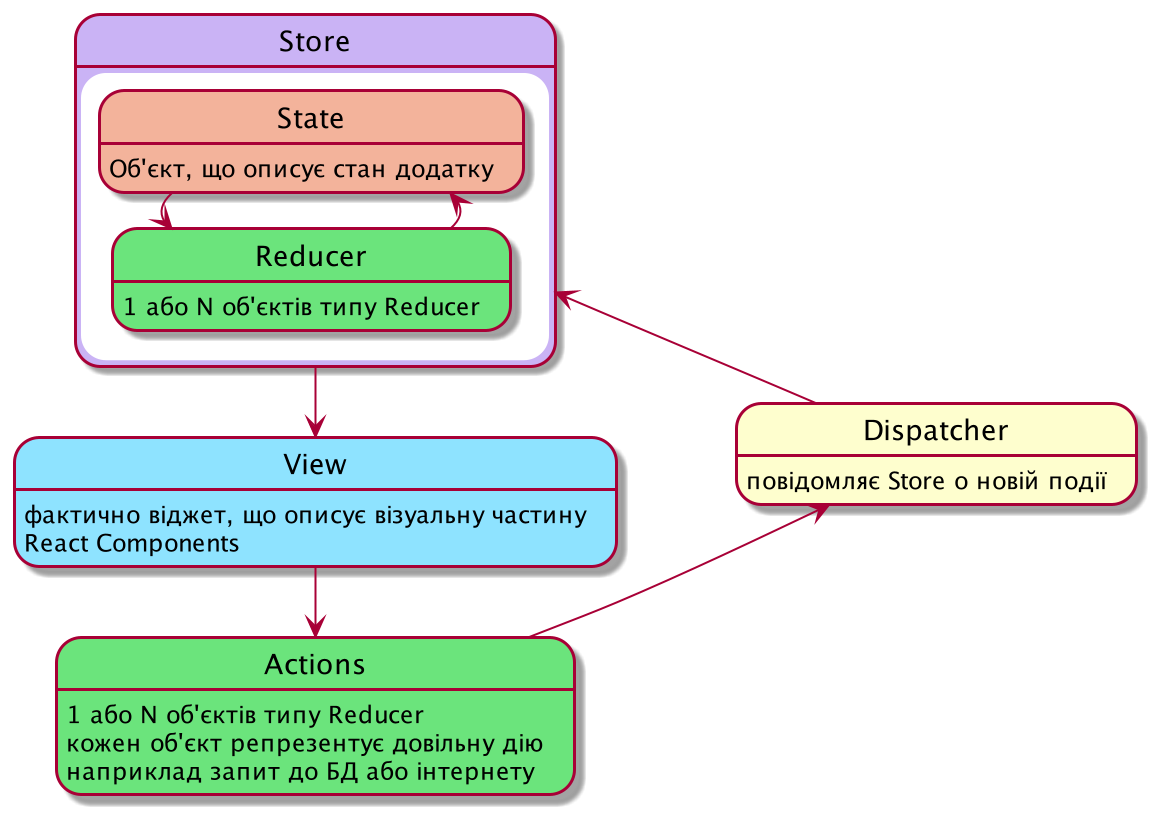
\includegraphics[scale=0.33]{redux.png}
        \caption{Схема Redux}
        \label{fig:rn_redux}
    \end{figure}
\end{center}

\subsection{Тестування в React Native}
\label{subsec:rn_testing}
У міру розширення вашої кодової бази невеликі помилки та крайні випадки, на які ви не очікуєте, можуть перетворюватися на більші збої.
Помилки призводять до поганого досвіду для користувачів і, зрештою, до втрат бізнесу.
Одним із способів полібшити якість сирцевого коду є написання тестів.

Одним з найкращих способів виправити помилку в коді є написання тесту, який виявляє її.
Потім, коли ви виправляєте помилку і повторно запускаєте тест, якщо він проходить, це означає, що помилка виправлена, і ніколи повторно не буде впроваджена в сирцевий код проекту.

Тести також можуть служити документацією для нових людей, які приєднуються до вашої команди.
Людям, які ніколи раніше не бачили кодової бази, аналіз тестів може допомогти зрозуміти, як працює існуючий код.
Нарешті, але не менш важливим є те, що більш автоматизоване тестування означає менше часу, проведеного за допомогою ручного контролю якості, звільняючи цінний час.

За замовчуванням React Native постачається з тестовою структурою Jest. \cite{jest_home_page}

\begin{lstlisting}[style=light, language=Python,label={lst:rn_jest_test},caption=Jest Unit Test]
  it('given 2 +2 returns 4', () => {
    expect(2 + 2).toBe('red');
  });
\end{lstlisting}

Jest дозволяє групувати тести з уживанням функцій "describe"(опис).
Підтримує хуки для ініціалізації стану "beforeEach"(перед кожним) та "beforeAll"(після всіх).

Unit test(єдносткові тести) допомагають протестувати тільки бізнес логіку.
Для тестування UI компонентів застосовується компонентне тестування.
Навіть якщо логіка вашого додатка має високий рівень охоплення тестуванням і є правильною,
без тестування компонентів ви все одно можете доставити непрацюючий інтерфейс для своїх користувачів.

Під час тестування компонентів React можна перевірити дві речі:

\begin{itemize}
    \begin{item}
        \textbf{Взаємодію:} для забезпечення належної поведінки компонента під час взаємодії з ним користувачем (наприклад, коли користувач натискає кнопку)
    \end{item}
    \begin{item}
        \textbf{Рендеринг:} щоб переконатися, що вихідний вигляд компонента, який використовує React, правильний (наприклад, зовнішній вигляд кнопки та розміщення її в інтерфейсі)
    \end{item}
\end{itemize}

Однак требу мати на увазі, що тестування компонентів - це лише тести JavaScript, що виконуються у середовищі Node.js.
Вони не беруть до уваги будь-який iOS, Android або інший код платформи, який підтримує компоненти React Native.
Звідси випливає, що вони не можуть надати вам 100\% впевненості, що все працює.
Якщо в коді платформи iOS або Android є помилка, вони її не знайдуть.

Останій клас тестів - це ті, що дозволяють протестувати в наскрізний спосіб наш додаток (далі E2E - End to End).
Це робиться шляхом запуску тестів на фінальній зборці додатку виконаному в середовищі Android або iOS.
У тестах E2E ви більше не думаєте про компоненти React, React Native API, Redux чи будь-яку бізнес-логіку.

Тести E2E дають вам максимально можливу впевненість у тому, що частина вашого додатка працює.
Однак в випадку E2E ми мусимо враховувати наступні компроміси.

\begin{itemize}
    \item їх написання займає більше часу порівняно з іншими типами тестів
    \item вони працюють повільніше
    \item вони більш нестабільні "flakky" ("flakky"  - це тест, який випадково проходить і не проходить без будь-яких змін в коді)
\end{itemize}

Доступно кілька інструментів тестування E2E.
\begin{itemize}
    \item у спільноті React Native Detox є популярним фреймворком, оскільки він спеціально підходить для додатків React Native.\cite{detox_home_page}
    \item ще однією популярною бібліотекою для iOS та Android додатків є Appium.\cite{appium_home_page}
\end{itemize}


\section{Фреймворк Flutter}
\label{sec:flutter}

\subsection{Flutter порівнняня віджетів з/без стану}
\label{subsec:flutter_widgets_theory}
Однією з основних тем, яка супроводжує вас під час використання Flutter, є те, що на 80\% розробки це потужне використання віджетів.

Віджети Flutter побудовані з використанням сучасного фреймворку, який черпає натхнення у React \cite{flutter_widgets_intro}.
Основна ідея полягає в тому, що ви створюєте свій інтерфейс з віджетів.
Віджети описують, як повинен виглядати їхній вигляд, враховуючи їх поточну конфігурацію та стан.
Коли стан віджета змінюється, віджет відновлює свій опис, при цьому фреймфорк порівнює новий стан з попереднім,
визначає мінімальні зміни, та оновлює дерево візуалізації, таким чином, переходячи з одного стану в наступний.

Головна структура будь-якого Flutter додатку будується на основі віджетів.
Згідно з специфікацією Dart першочергове, що ми робимо це імпортоування компенентів за допомогою конструкції \textbf{import}.
Наступними кроками буде ініціалізація в \textbf{main()} функції дерева віджеті \textbf{WidgetsFlutterBinding.ensureInitialized()} та
виклик функції \textbf{runApp()}, що прив'язує визначене нами дерево віджетів.

Далі ми наводимо сирцевий код, що описує логіку ініціалізації додатку та визначає головний віджет додатку. \ref{lst:flutter_app_widget}
Як ми бачимо з наведеного сирцевого коду, по суті, розробка в Flutter подібна до гри з матрьошкою,
де ми вкладаємо один віджет в настуапний поступово додаючи складність до розвязання.

Треба звернути увагу, що головний віджет не має стану і тим самим визначає, що кореневий віджет буде не змінним
під час перерахування дерева після зміни стану в інших шарах додатку.

Тепер ознайомившись з прикладом віджету без стану, слід навести протилежність, а саме StateFullWidget(зі станом).
Ми зробимо це на прикладі списку котрий відображає додаток. \ref{lst:flutter_app_widget}

Головне, що требу розуміти в випадку віджетів зі станом це те, що зміна стану приводить до перемалювання віджету.
Оскільки один віджет може повертати довільно складне дерево віджетів змінивши стан голови гілки призведе до змін
ланки віджетів, що наслідує наш віджет зі станом.

\subsection{Система побудування з використанням Flutter CLI}
\label{subsec:flutter_cli_theory}
Flutter CLI - інструмент командного рядка котрий дозволяє створити, виконати, зібрати сирцевий код проектів фреймфорку Flutter.

\begin{lstlisting}[style=light, language=Python,label={lst:flutter_cli_create},caption=Flutter Create Project]
flutter create my_app
cd my_app
flutter analyze
flutter test
flutter run lib/main.dart
\end{lstlisting}

Як видно в лістингу \ref{lst:flutter_cli_create} ми виконуємо команду, що створює, перевіряє, запускає тести та відтворює фактично код додатку.

Додатково набір інсрументів дозволяє завантажити, сконфігурувати та під'єднати транзитивні залежності проекту \ref{lst:flutter_pub}.
\begin{lstlisting}[style=light, language=Python,label={lst:flutter_pub},caption=Flutter Dependency Resolution]
flutter pub get
flutter pub outdated
flutter pub upgrade
\end{lstlisting}

Повний список залежностей можна знайти на офіційній веб сторінці \cite{flutter_cli}.

\subsection{Flutter та пакет http.dart}
\label{subsec:flutter_http_dart_theory}
Отримання даних з Інтернету необхідно для більшості програм.
На щастя, Dart і Flutter надають інструменти, такі як httpпакет, для цього виду робіт.

Цей пакет містить набір функцій та класів високого рівня, що полегшують споживання ресурсів HTTP.
http.dart підтримує мобільну, настільну та браузерні платформи.

Використання функцій верхнього рівня дозволяє робити окремі HTTP-запити.
Якщо є потреба робити кілька запитів на один і той же сервер, тоді зручніше всього тримати відкритим постійне з’єднання,
використовуючи клієнт, а не одноразові запити.

\begin{lstlisting}[style=light, language=Python,label={lst:flutter_pub},caption=Flutter Dependency Resolution]
import 'package:http/http.dart' as http;
var client = http.Client();
try {
  var uriResponse = await client.post(Uri.parse('https://example.com/whatsit/create'),
      body: {'name': 'doodle', 'color': 'blue'});
  print(await client.get(uriResponse.bodyFields['uri']));
} finally {
  client.close();
}
\end{lstlisting}

В нашому додатку запит до інтернету описан в наступному описі сирцевого коду \ref{lst:flutter_networking}.

Найголовнішим принципом, котрим ми опируємо в прикладі запиту до інтернету, це використання "обіцянок" на базі dart:async Future<T>.
Асинхронні операції дозволяють нашій програмі завершити роботу, чекаючи закінчення іншої операції.
Результат використання Future API або закінчиться в завершенному стані або незавершенному.

Коли ми вперше виконуємо асинхрону функцію, то отримаємо посилання на незавершену дію, з якої ми очікуємо результат або помилку.
Щоб уникнути розповсюдження помилки до верхнів шарів ми маємо використати try/catch синтаксис.

Як видно з нашого прикладу використання пакету http.dart в по'єднанні з dart:async дає зручне
та швидке розв'язання проблеми створення та прослухання результатів з інтернету.

\subsection{Flutter та пакет sqflite}
\label{subsec:flutter_sqflite_theory}
SQFlite - це порт SQLite драйверу для платформ написаних на Dart, яке підтримує iOS, Android та MacOS.

До можливостей sqflite можна віднести:

\begin{itemize}
    \item Підтримка транзакцій та пакетів.
    \item Помічники для вставки / запиту / оновлення / видалення запитів.
    \item Операції до БД, виконуються у фоновому потоці на iOS та Android.
    \item Підтримка Linux / Windows / DartVM за допомогою sqflite_common_ffi.
\end{itemize}

Рішення, що використовує цю бібліотеку можна знайти за наступним посиланнєм \ref{lst:flutter_sqflite}.

Для того щоб, уникнути витік залежності рішення SQFlite було огорнуто в додатковий тип \textbf{BreedDatabase}.
\textbf{BreedDatabase} дає можливість виконання стандартних процедур підключення до БД з розширенням .sqlite
на стандартному шляху до файлу абстрагованого за допомогою \textbf{getDatabasesPath()} API.

Оскільки наша огортка, це вікно в SQL світ, то наш додаток здатен виконувати всі доступні із стандартного набору
SQL операції.

\subsection{Управління станом в Flutter}
\label{subsec:flutter_state_app}
Flutter пропонує кілька способів для управління станом. Серед них BLoC, Provider, Statefull Widgets, InheritedWidgets.
В даній роботі ми розглянемо Provider API, котрий взяв за основу систему InheritedWidgets(віджет, що наслідує).
Для того щоби зрозуміти контроль стану з Provider API ми повинні розлянути:

\begin{itemize}
    \item ChangeNotifier - це простий клас, включений до Flutter SDK, який забезпечує повідомлення про зміни своїх слухачів. Іншими словами, якщо щось є ChangeNotifier, ви можете підписатися на його зміни.
    \item ChangeNotifierProvider - це віджет, який надає екземпляр ChangeNotifier своїм нащадкам. Це походить від пакету провайдера.
    \item Consumer - це віджет, що дозволяє нам огорнути будь-який інший віджит далі в ієрархії та зчитати стан з класу, що наслідує ChangeNotifier.
\end{itemize}

В нашому додатку ми використали StateNotifier, котрий обновлює всіх підписників стану.
Так наприклад зміна значення з стану "завантажується" на стан "завантажений" приводить до перебудови віджету \ref{lst:flutter_sqflite}.

\subsection{Юніт тестування в Flutter}
\label{sec:flutter_unit_testing_app}
Як було вже зазначено, найкращий спосіб контролю якості в проекті це написання та сопроводження коду написанням юнит тестів.
Цей підхід до розробки програмного забезпечення не оминув і розробку під Flutter.

В даній секції ми наведемо приклад тесту написаного для коду бізнес логіки \ref{lst:flutter_unit_test}.
Ми застосуємо пакети test та mockito.
Пакет тест надає доступ до функцій, які дозволяють нам групувати тести.
Пакет mockito надає функціонал, що дозволяє конфігурувати поведінку об'єктів типу mock(заглушка).

Ми маємо дві "рухомі" залежності: шар комунікації з мережею та БД.
Рухомі частини - це те що ми, як користувачі бібліотек http.dart та SQFlite не контролюємо.
Отже, щоб спростити конфігурацію юніт тестування ми замінили реальні об'єкти на об'єкти заглушки.


\section{Фреймворк Kotlin Multiplatform (KMM)}
\label{sec:kmm}

\subsection{UI та Kotlin Multiplatform}
\label{subsec:kmm_ui}
Специфіка розробки з використанням Kotlin Multiplatform передбачує, що розробка рівня UI буде досягнута
інструментами нативними для платформи.

Для розробки UI під Android використовується декларативний XML, що відтворюється під час виконання в середовищі компоненту
контейнера так званої Activity(активність) (див. \ref{lst:android_xml}).

Нещодавно з'явився тренд розробки UI з уживанням
Kotlin DSL(Domain Specific Language - Специфічна Мова Домену) так званий Jetpack Compose \cite{jetpack_compose}.

Як видно з прикладу \ref{android_jetpack_compose} Android екосистема взяла той самий керунок, що Flutter та React Native.
Такий самий тренд можна спостерігати і в розробці під iOS, де декларативний синтаксис описується з Swift UI \cite{swift_ui}.

Як видно з прикладів \ref{android_jetpack_compose} та \ref{ios_swift_ui} Android та iOS теж вибрали стежку декларативної розробки UI.
В свою чергу стає зрозуміло, що Kotlin Multiplatform не розв'язує проблему спільної бази коду для коду UI.
Це дуже важливий момент, оскільки весь UI треба дуплікувати під кожну платформу.
Якщо Kotlin Multiplatform не розв'язує проблему, то для чого його використовувати?
Задачу яку собі поставив Kotlin Multiplatform, це опис спільної логіки, тобто звернення до бази даних, файлової системи, інернету, тощо.

\subsection{Система побудування Gradle та Kotlin Multiplatform}
\label{subsec:kmm_gradle}

Gradle - це система побудування проектів розроблена для рішення проблем побудування проектів зокрема для JVM платформ.
Gradle - це інструмент автоматизації збірки з відкритим кодом, орієнтований на гнучкість та продуктивність. \cite{gradle_user_manual}
Сценарії збірки Gradle пишуться із використанням DSL Groovy або Kotlin. \cite{gradle_user_manual}

Оскільки Kotlin спочатку був розроблен для JVM систем, то був на раніх етапах інтегрован в екосистему.
З розвитком Kotlin Multiplatform дана система була наслідувана і надалі використовується для побудування крос-платформеного проекту.

Якщо ви знайомі з проектами Android, то знаєте, що залежності та конфігурація побудування проекту можна знайти у build.gradle.

Оскільки shared модуль є бібліотекою для Android, він також містить власний build.gradle скрипт, де описані залежності.
Скрипт "shared/build.gradle.kts", описує конфігурації сирцевих кодів з використанням sourceSets, що відповідає каталогам у спільному проекті.

Кожна частина бібліотеки, оголошує власні залежності в визначених наборах джерел.
Наприклад, бібліотека параметрів мультиплатформних налаштувань оголошується лише у commonMain та commonTest,
оскільки бібліотека використовує метадані gradle для виведення залежних від конкретних платформ залежностей.
Інші бібліотеки, які залежать від реалізації платформи, наприклад SqlDelight, вимагають конфігурації яка задовольнить
умовам середи виконання.

Наприклад для sourceSet commonMain визначена залежність з пакету sqlDelight.runtime, а в androidMain sqlDelight.driverAndroid.

\subsection{Комунікація з мережею в KMM http.dart з ktor та couroutines}
\label{subsec:kmm_ktor}
На даний момент серед кроссплатформених бібліотек, що дозволяє нам моделювання інтернет викликів,
найпоширенішою - є розв'язання Ktor \cite{ktor_home_page}.
В додатку коду, що йде нижче \ref{kmm_ktor} ми розглянемо приклад реалізації клієнта,
що надалі створює з'єднання з API сервісом, що повертає нам список порід собак.

Визначаємо інтерфейс, що повертає нам результат виконання виклику до API \ref{lst:kmm_ktor}.

Важливим момент є те, що функція визначена ключовим словом \textbf{suspend}.
\textbf{suspend} маркерує нашу функцію, як ту, що буде виконувати "блокуючу" операцію.
Виконання викликів до інтернету операція дорога і можевиконуватися секундами.
Створюємо об'єкт Ktor клієнта та конфігуруємо Json Serializer/Deserializer.
\textbf{ensureNeverFrozen} гарантує, що freezing(заморожування) закінчиться помилкою FreezingException.
Дозволяє уникнути небажаного ефекту freezing, що є основою безпечного контролю посилань між паралельними потоками
під час виконання програмою асинхроних викликів.
Реалізуємо функцію інтерфейсу декларуючи посилання, що нам поверне результат.

Як ми бачимо реалізація виклику за допомогою Ktor та Kotlin, хоча виглядає громоздко, але не є складною.
Більшість логіки, що створює сокет і опрацьовуі потік байтів схована за публічним інтерфейсом.
Від клієнта потребується декларування викликів та дизайн DTO(Data Transfer Object - Транспортний Об'єкт Даних),
в нащому випадку це клас, що описує структуру Json відповіді BreedResult.

\subsection{Комунікація з БД в KMM з SQLDelight}
\label{subsec:kmm_sqldelight}
Для роботи з БД в нашому KMM(Kotlin) проекті було використана SQLDelight \cite{sqldelight_home}.
SQLDelight використовує ідею генерації коду для клієнту на основі SQL визначень описаних в окремому файлі.

Як видно в прикладі з додатку \ref{table_sq_gen} спочатку ми описуємо структуру таблиць за допомогою SQL.
Далі ми надаємо інструкцію \textbf{selectAll}, що буде використана SQLDelight для генерації коду \ref{lst:table_sq_gen}.

Результатом виконання SQL запиту буде посилання на об'єкт типу курсор, що дозволяє в динамічний спосіб зчитати
результат та адуптувати результат до конкретного типу. Таким чином, ми уникаємо написання низькорівневого коду,
в якому дуже просто припуститися помилки. В випадку більш складних схем БД перевага згенерованого коду дозволяє
нам уникати надмірного повторення в написанні коду прослойки для коммунікації з БД.

\subsection{Юніт тестування в KMM додатку}
\label{subsec:kmm_unit_testing}

Як і в випадку інших платформ розробки тестування коду є критичною для розвитку продукту.
KMM і тут не відстає і пропонує розв'язання для тестування.
Оскільк Kotlin підтримує JVM(Java Virtual Machine) середовище ми можемо запускати тести на стороні Linux, Windows та MacOS платформ.

Тести, що супроводжують загальну логіку тримають в відокремленому репозиторії commonTest.
Для конфігурації специфічного для платформи коду виділяють iosTest для iOS та androidTest для Android платформ.

В нашому додатку був написаний простий інтеграційний тест (див. \ref{lst:kotin_test_common}).
Дуже важливо підкреслити наявність ф-цій \textbf{testDbConnection} та \textbf{runTest}.
Де \textbf{testDbConnection} абстрагує реалізацію драйверу підключення до БД та буде реалізована для кожної
з платформ в своєму специфічному вихідному наборі (ios, android).
\textbf{runTest} абстрагує реалізацію логіку запуску тесту.
Модель багатопотоковість унікальна для кожної з платформ, тому впроваджується абстракція та конкретна імплементація
для кожної з платформ.

Важливо зауважити, що ми базуємо наше рішення на базі специфічної для KMM пари \textbf{expect} та \textbf{actual}.
Дані ключові слова маркерують ф-ції, як ті що залежать від API специфічного для платформи.

В \ref{lst:kotin_test_ios} ми використовуємо в якості реалізації драйвер специфічний для iOS платформи.

В \ref{lst:kotin_test_android} ми використовуємо в якості реалізації драйвер специфічний для Android платформи.

З наведених приклавдів можно зробити висновок, що KMM намагається максимально тісно співпрацювати з API специфічний для платформи.
Таке рішення потребує знання не тільки специфіки Kotlin але й розуміння бібліотек специфічних для платформ.
Тобто KMM не будує додатковий рівень абстракції, що ховає доступ до конкретних специфікацій.
